% ------------------------- MAIN TASK ---------------------------------
\section{Main task}
\subsection{Schematic proposal for limiting output current to 250mA} \label{ssec:num11}
{
	We were asked to design a proposed scheme to limit the output current to 250mA, to do this we decided to change the principle of the connections to create a current source using the LM317.	
	
	\begin{figure}[h]
		\centering
		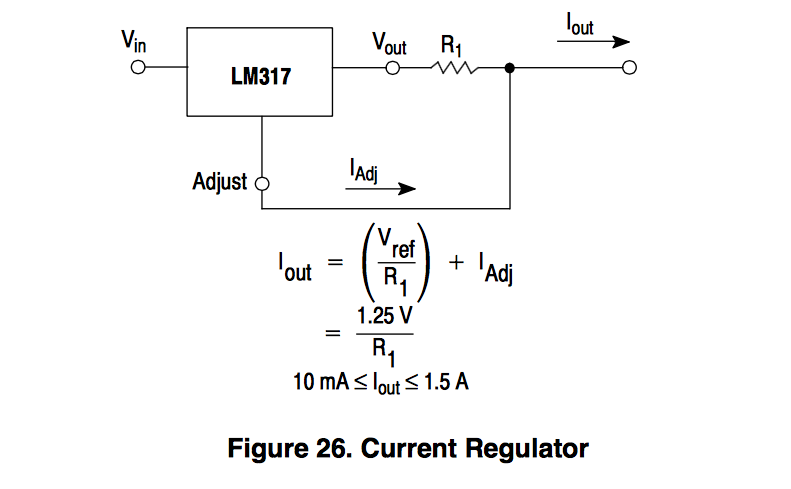
\includegraphics[width=0.7\linewidth]{../Figures/Partie2/SourceCourant}
		\caption{Current source with LM317}
		\source{Stackexchange "lm317-µa-constant-current-source-possibility"}
		\label{fig:sourcecourant}
	\end{figure}
	
	We use the reference voltage (\textbf{1.25V}) of the internal diode, so the output current depends on the resistance \textbf{R1} plus the leakage current of the diode.
	
	By adding and changing a load resistor in the circuit, the induced output current will vary, as will the voltage, but the current will not exceed : \\ $\frac{Vref}{R1}+I_{ADJ}$ \vspace{+6pt}
	
}

\newpage
\subsection{Plotting output tension depending on output current} \label{ssec:num12}
{
One of the unique features of the LM317 is its ability to automatically adjust its output voltage in response to changes in temperature. This is accomplished using a built-in temperature-sensing circuit that monitors the temperature of the LM317 and adjusts the output voltage accordingly.\vspace{+12pt}

When the temperature of the LM317 increases, the temperature-sensing circuit will cause the output voltage to decrease slightly. This helps to prevent the LM317 from overheating and ensures that it continues to operate within safe temperature limits. Similarly, when the temperature of the LM317 decreases, the temperature-sensing circuit will cause the output voltage to increase slightly. This helps to maintain a stable and consistent output voltage, even in changing temperature conditions.\vspace{+12pt}

Overall, the LM317's ability to regulate according to temperature makes it a versatile and reliable choice for applications that require a constant output voltage, such as in power supply circuits and battery chargers. \vspace{+12pt}

We will observe this characteristic through our following measurements.

\subsubsection{List of all the instruments}

\begin{tabular}{l | l | l}
	Instrument & Designator & Reference \\ 
	\hline\hline & & \vspace{-8pt}\\ 
	Oscilloscope & P1 & ES.SLO2.05.01.08 \\
	Current probe & P2 & ES.SLO1.00.06.04 \\
	DC power supply & G1 & ES.SLO2.00.00.31 \\
	Electronic load & G2 & ES.SLO2.00.02.60 \\
	Waveform generator & G3 & ES.SLO2.00.00.138 
\end{tabular}

\clearpage

\subsubsection{Measures}
\underline{Measurement schematic:}
\begin{figure}[h]
	\centering
	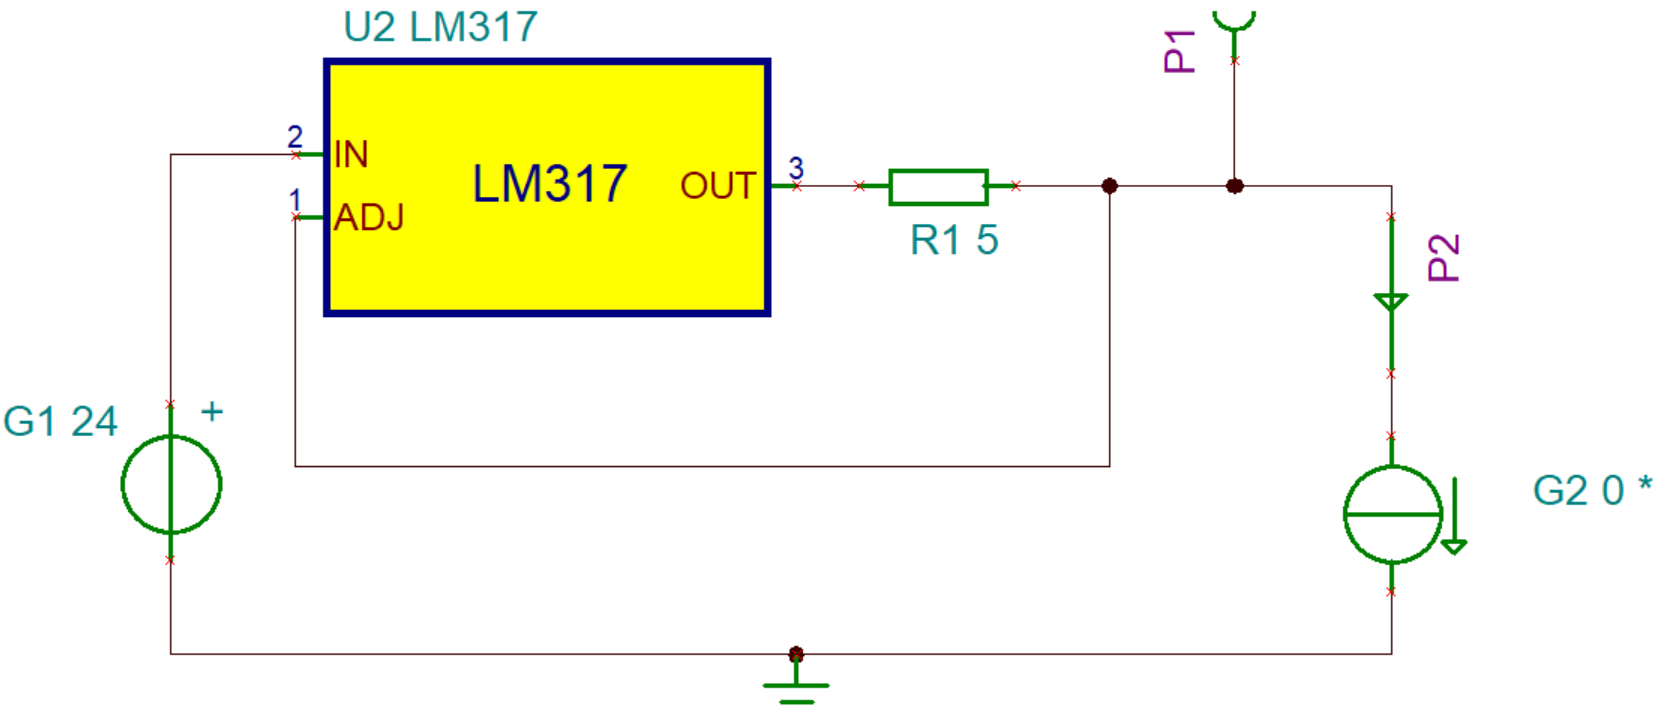
\includegraphics[width=0.6\linewidth]{../../SchemaMesureChargeElectronique}
	\caption{Measurement schematic for output voltage depending on output current}
	\label{fig:schemamesurechargeelectronique}
	\source{Authors}
\end{figure}

\underline{Measurement method:}

In order to perform the requested measurements, we had to change the induced current of the electronic load at each iteration, with a step of 10mA, and measure the current and voltage.\vspace{+6pt}

\underline{Measures:}
\begin{figure}[h]
	\centering
	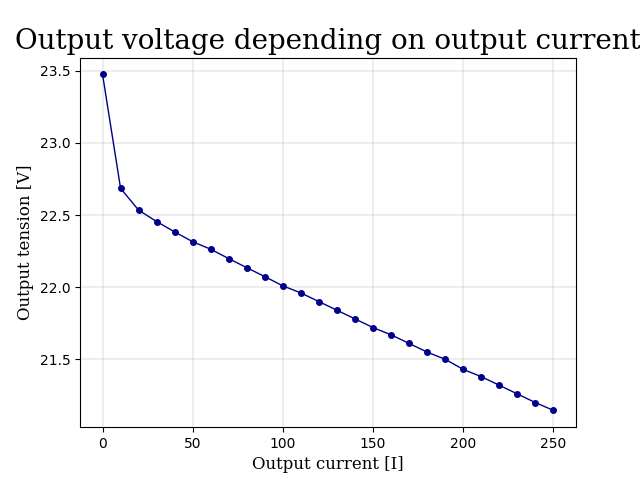
\includegraphics[width=0.7\linewidth]{../../Grph-pointG}
	\caption{Point G measurements}
	\label{fig:grph-pointg}
	\source{Authors}
\end{figure}

\clearpage
\underline{Analysis:}

As we can see on figure \ref{fig:grph-pointg}, When no current is inducted on the output, the potential voltage on the load is at its maximum (\textbf{$\sim 24V = \sim Vin$}). We can see that when a larger current is induced, the voltage drops, which is mainly due to the voltage loss on the serial resistor. We also noticed during the measurements that when the electronic load is short-circuited, we have an output current of \textbf{255mA} (which is slightly higher than our sized maximum) and an output voltage of \textbf{0V}.

\subsubsection{Simulation}

The simulation schematic is the same as the one in figure \ref{fig:schemamesurechargeelectronique}.

\underline{Results:}
\begin{figure}[h]
	\centering
	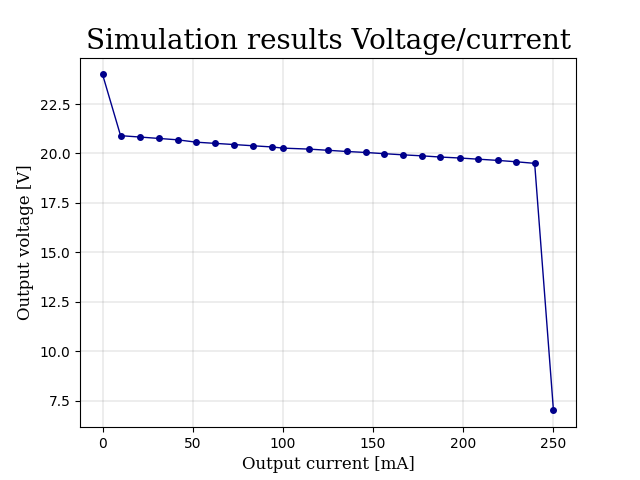
\includegraphics[width=0.7\linewidth]{../../Simu-pointG}
	\caption{Simulation results}
	\label{fig:simu-pointg}
	\source{Authors}
\end{figure}

\underline{Analysis:}\vspace{+6pt}

We can see that the simulation results are similar to our previous measurements, except that the delta between the highest and lowest voltage is smaller in the simulation, probably because the simulation does not take into account all the hardware contingencies.

}

\newpage
\subsection{Oscillogram of the output current depending on the output tension} \label{ssec:num13}
The internal temperature-sensing circuit that monitors the chip's temperature can also adjusts the amount of time that the regulator is on to maintain a stable output voltage, and we will observe this feature under this section.
{
	\subsubsection{Measurements}
	\underline{Schematic:}
	\begin{figure}[h]
		\centering
		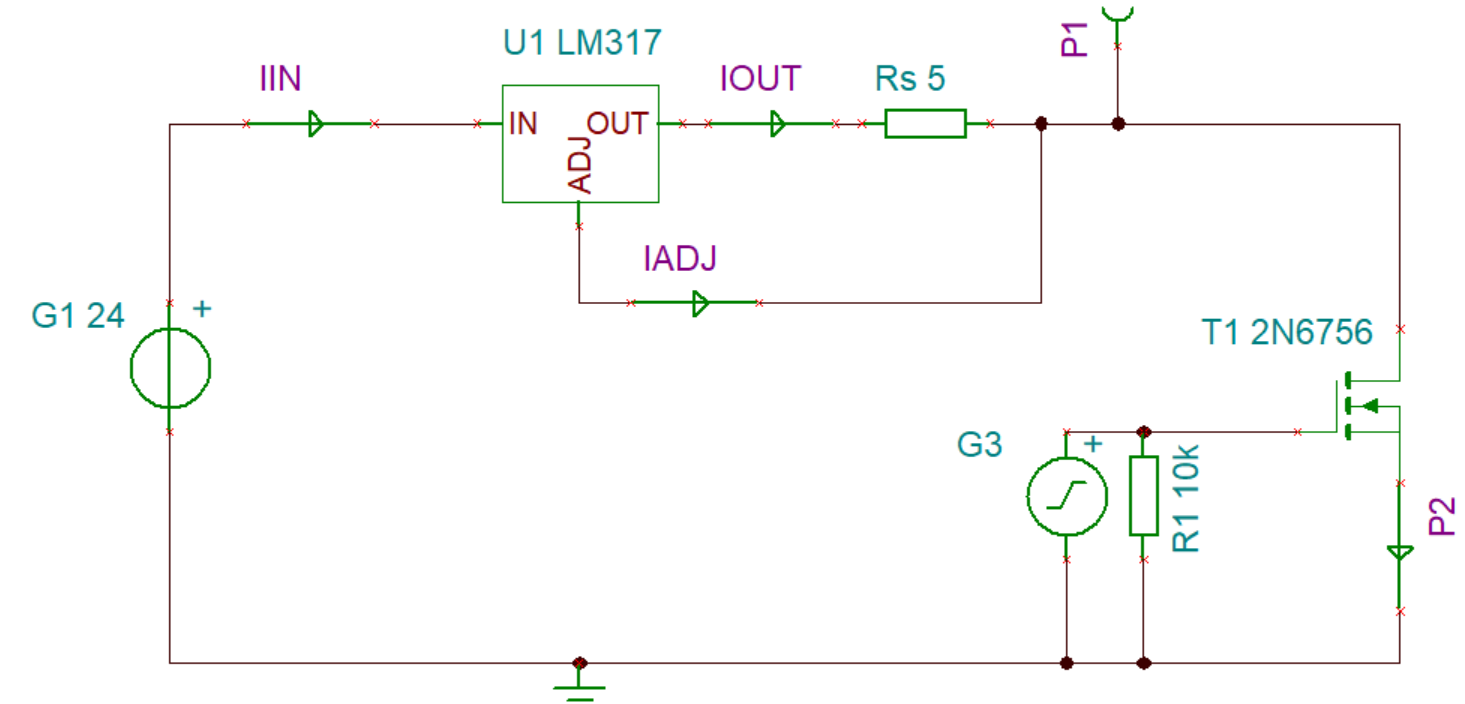
\includegraphics[width=0.5\linewidth]{../../schemaMesurePulses}
		\caption{Measurement schematic}
		\label{fig:schemamesurepulses}
		\source{Authors}
	\end{figure}

\underline{Measure:}
\begin{figure}[h]
	\centering
	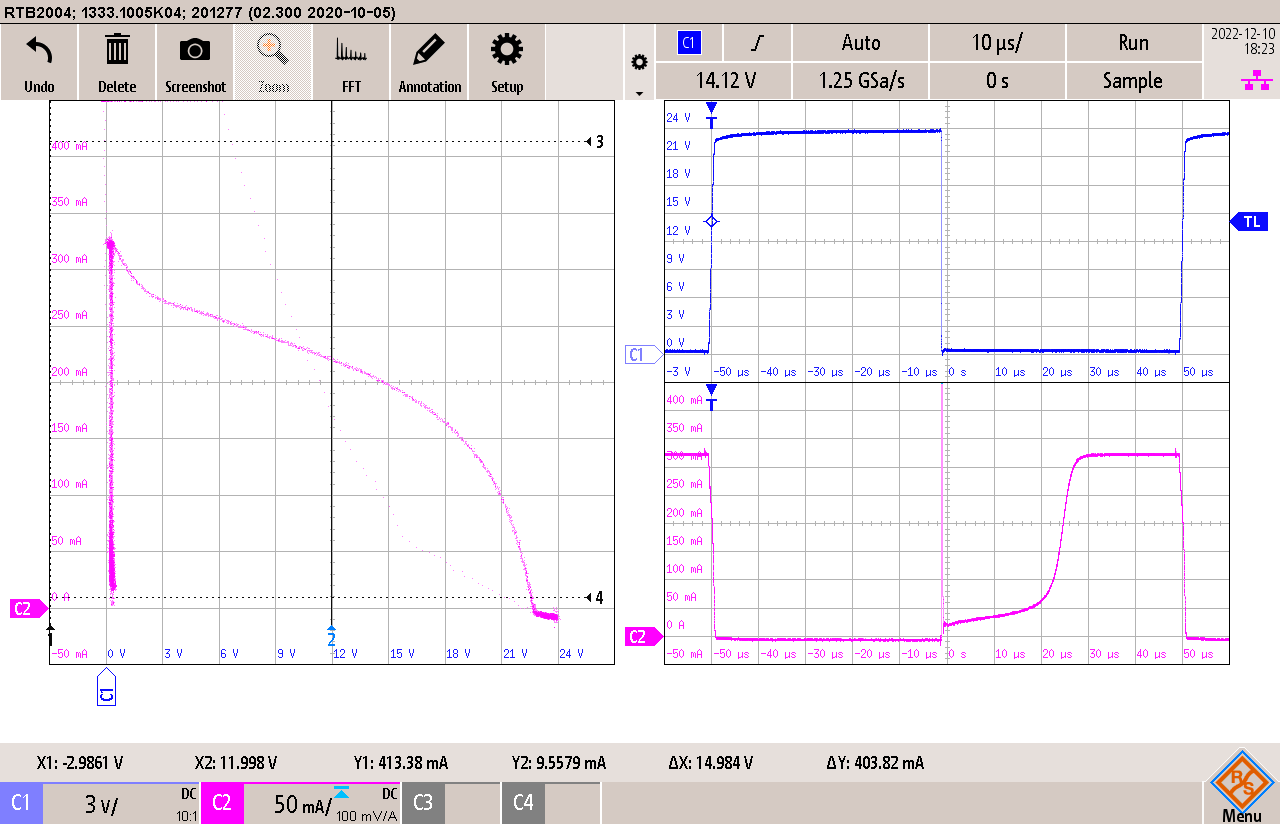
\includegraphics[width=0.5\linewidth]{../../mesure_osciollogramme}
	\caption{Oscillogram}
	\label{fig:mesureosciollogramme}
	\source{Authors}
\end{figure}


\underline{Analysis:}

We can see on the figure \ref{fig:mesureosciollogramme}, when no heat sink is used, that the LM317 adjusts the amount of current supplied to the load, in order to maintain a stable output voltage over time. By adding a heat sink to the TO-220 package, the output current supplied increases more rapidly when the MOSFET switches. 

\clearpage
\subsubsection{Simulation}
\underline{Results:}

\begin{figure}[h]
	\centering
	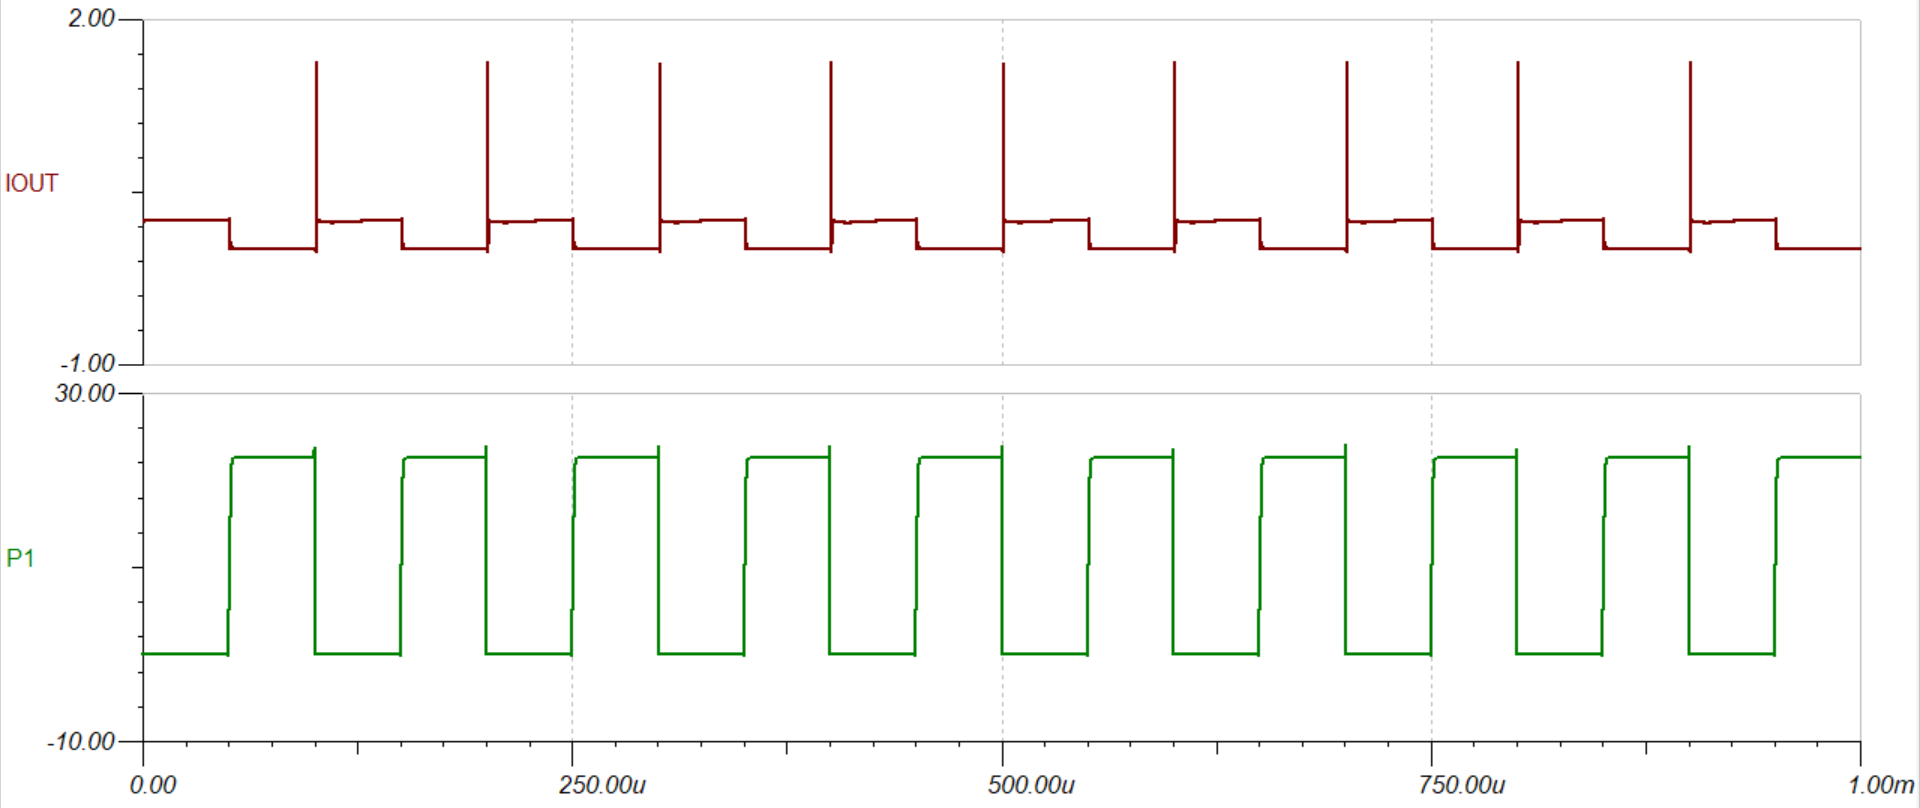
\includegraphics[width=0.9\linewidth]{../../Simulations/Simu-Switching}
	\caption{Simulation results}
	\label{fig:simu-switching}
	\source{Authors}
\end{figure}
\underline{Simulation analysis:}

We can see that the simulation does not take into account the heating of the component, because the output current is always ON when the mosfet conducts, which means that the internal temperature sensor and control is not simulated. What is similar to the measures is the current peak when switching, it is certainly due to a capacitive phenomenon. 


}

\clearpage

\subsection{Dissipated power calculation} \label{ssec:num14}
{
	We can calculate the power dissipated in the LM317 using the same formula as before and taking in consideration the duty cycle. \\
	$\alpha = 50\% $ \\
	
	\begin{equation}
		P_{reg_{ON}} = (U_{in_{ON}} - U_{out_{ON}})*I_{out_{ON}}
	\end{equation}
	
	\begin{equation}
		P_{reg_{OFF}} = (U_{in_{OFF}} - U_{out_{OFF}})*I_{out_{OFF}}
	\end{equation}
	
	\begin{equation}
		P_{reg_{TOT}} = P_{reg_{ON}}*\alpha + P_{reg_{OFF}} * (1-\alpha)
	\end{equation}
	
	Calculated values for our application:\\
	$ P_{reg_{ON}} = 6 W $ \\
	$ P_{reg_{OFF}}  = 0 W $ \\
	$ P_{reg_{TOT}} = 3 W $ \\
	
	Datasheet set the maximum allowable power dissipation as : \\
	
	\begin{equation}
		P_{MAX} = (T_{J_{MAX}} - T_{A}) / Rth_{JA}
	\end{equation}

	In our case, this value is :
	
	\begin{equation}
	P_{MAX} = 3,03 W
	\end{equation}

	So this mean we reached the absolute maximal power that our LM317 can dissipate. Going higher than this value would impact reliability and/or trigger temperature protections.

}

\clearpage

\subsection{Estimation of the junction's temperature without cooling} \label{ssec:num15}
{
	$ T_{A} = 35 \ °C $ \\
	$ Rth_{JA} = 37.9 °C/W $\\
	We can define the temperature of the junction by :
	\begin{equation*}
		T_{J} = T_{A} + Rth_{JA} * P_{reg_{TOT}}
	\end{equation*}
	
	Calculated value for our application:\\
	$ T_{J} = 148,7 \ °C $ \\
	
	The datasheet set the maximal admissible temperature to 150°C.
}
\subsection{Short-circuited output - dissipated power calculation} \label{ssec:num16}
{
	When short-circuiting the output, we get the maximal current possible. As the output is grounded, all the voltage occurs in the LM317. This leads to a situation where the LM317 needs to dissipate a lot of power, which we calculated this way : \\
	
	\begin{equation}
		P_{reg} = (U_{in} - U_{out} ) * I_{out}
	\end{equation}

	Calculated values for our application:\\
	
	$ P_{reg} = 6W $ \\
}

\clearpage
\section{Conclusion}
{
	In this practicum we learned how to configure and use a circuit based on the LM317 regulator. \\
	We first established the way of using it as a voltage regulator. We needed to take in consideration the ADJ current that was neglecated by the datasheet to fit to our specific application. We then made sure that our sizing was correct. We then simulated our circuit to confirm that, which was working as expected by specifications.\\
	Secondly, we used the LM317 as a current limitator. We found a schematic in the datasheet composed of only a single resistor. We made sure that the current limitation was working by short-circuit the output. We then made some measurement to observe the change in the output voltage in comparaison with output current. We made sure that the LM317 could handle all the power dissipation by calculating it. We saw that the circuit was at its maximum capabilities and even exceed it sometimes which triggered its internal protections.\\
	
	\vspace{90mm}
	\begin{tabular}{@{}p{2.5in}p{2in}p{2in}@{}}
		
		\hrulefill && \hrulefill\\
		Miguel Santos && Ali Zoubir\\
		ETML-ES \\
		Lausanne, 11.22.2022 \\
	\end{tabular}
}

\clearpage